\chapter{Peking}
\section{Type 3}
\begin{figure}[htbp]
\centering
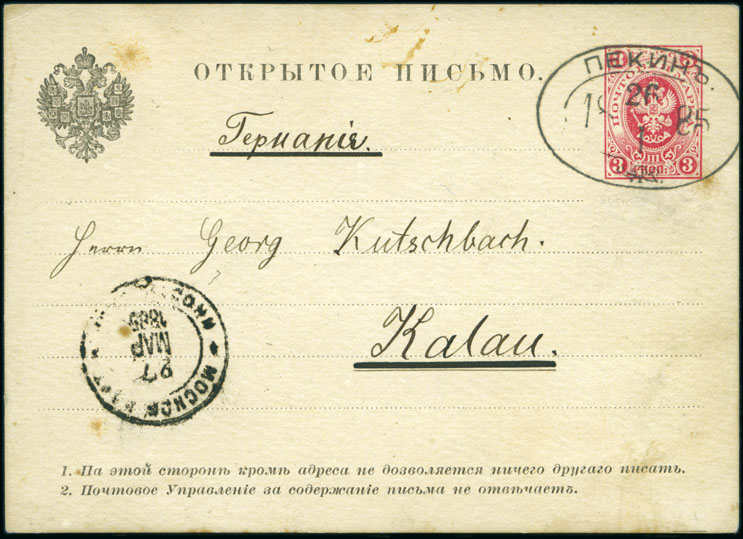
\includegraphics[width=.95\textwidth]{../russian-post-offices-in-china/10024.jpg}
\caption{
10024 PEKING: 1885 3k Postal stationery card sent from the German Embassy in 
Peking to Kalau, Germany, cancelled by double oval Peking 26.1.85 ds 
(T\&S type 3 variety day above month), Moscow transit, couple of tone 
spots otherwise fine, an extremely rare postal marking
\euro 20,000.00 
}  
\end{figure}

\begin{figure}[htbp]
\centering
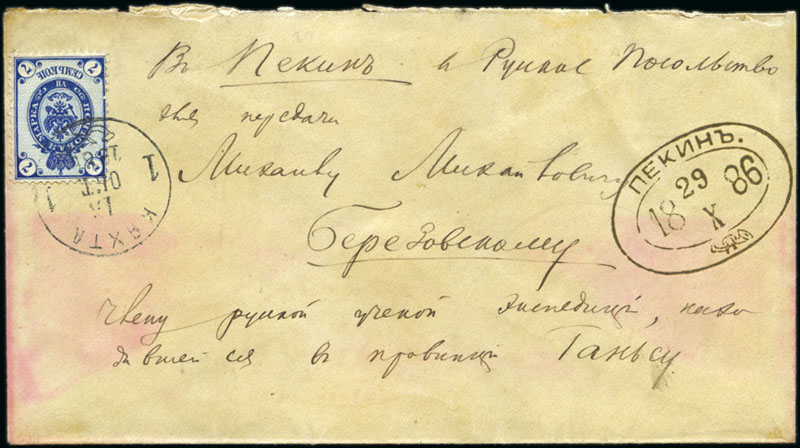
\includegraphics[width=.95\textwidth]{../russian-post-offices-in-china/10025.jpg}
\caption{
10025	PEKING INCOMING: 1886 Cover from Kyakhta (Siberia) to
the Russian Embassy in Peking, with Arms 7k tied by Kyakhta cds and double
oval Peking 29.10.86 ds (T\&S type 3 variety day above month) adjacent upon arrival
\euro 700.00
}  
\end{figure}
                                                                                      